\hojaejercicio{Parte 1: Capítulo 1}
% Ajustamos el contador para que el primer ejercicio sea el 2, coincidiendo con el PDF original
\setcounter{ejercicio}{1}

% Ejercicio 2
\ejercicio{resuelto}{}{
    Dado un entero $N \in \N$, $N \ge 1$, y $N^2$ funciones continuas $a_{ij} \in \mathcal{C}(\R; \R)$, con $i,j \in \{1, \dots, N\}$, considera el problema de Cauchy
    \[
        \begin{cases}
            u_i' = \sum_{j=1}^N a_{ij}(t) \cos u_j, \quad i \in \{1, \dots, N\}, \\
            u(t_0) = u_0.
        \end{cases}
    \]
    Demuestra que, para todo $t_0 \in \R$ y $u_0 \in \R^N$, admite una única solución $u(t; t_0, u_0)$, definida globalmente para $t \in \R$.
}{
    Escribimos el sistema de forma vectorial:
    \[
        u' = f(t,u) \implies \begin{pmatrix} u_1' \\ \vdots \\ u_N' \end{pmatrix} = \left( \sum_{j=1}^N a_{ij}(t) \cos u_j \right)_{1 \le i \le N}
    \]
    
    Analizamos la matriz Jacobiana $D_u f(t,u)$:
    \[
        D_u f(t,u) = \left( \frac{\partial f_i}{\partial u_j} (t,u) \right)_{1 \le i,j \le N} = \left( -a_{ij}(t) \sin u_j \right)_{1 \le i,j \le N}
    \]
    
    Por ser $f$ de clase $\mathcal{C}^1$ respecto a $u$, sabemos que es localmente Lipschitziana. 
    Para acotar la constante de Lipschitz, acotamos la norma de las derivadas parciales. Si tomamos cualquier intervalo compacto de tiempo $J = [\alpha, \beta] \subset \R$:
    \[
        \left| \frac{\partial f_i}{\partial u_j} (t,u) \right| = \left| -a_{ij}(t) \sin u_j \right| \le |a_{ij}(t)| \le \|a_{ij}\|_{\infty, J} \quad \forall u \in \R^N
    \]
    Como la derivada está acotada globalmente en $\R^N$ para $t \in J$, deducimos que $f$ es globalmente Lipschitziana respecto de $u$ uniformemente en subintervalos compactos de tiempo.

    Para demostrar la existencia global, tomemos una sucesión de intervalos compactos expansivos:
    \[
        J_n = [t_0 - n, t_0 + n], \quad n \ge 1
    \]
    Por el Teorema de Cauchy-Lipschitz Global en $J_n$, existe una única solución $u_n(t)$ definida en $J_n$. 
    Además, por la unicidad de las soluciones, las restricciones deben coincidir: $u_{n+1}|_{J_n} = u_n$ (ya que de lo contrario se contradiría la unicidad en $J_n$).

    Dado cualquier $t \in \R$, $u(t)$ estará definida porque siempre podemos encontrar un $n$ suficientemente grande tal que $t \in [t_0 - n, t_0 + n]$. Esto nos permite definir la solución en todo $\R$ como el límite:
    \[
        u(t) = \lim_{n \to \infty} u_n(t)
    \]
    
    Supongamos por reducción al absurdo que no fuera única. Entonces existiría otra solución $\tilde{u}$ y un instante $\tilde{t}$ tal que $u(\tilde{t}) \neq \tilde{u}(\tilde{t})$. Sin embargo, podemos tomar $n$ suficientemente grande de forma que $\tilde{t} \in J_n$. Al restringir ambas soluciones a $J_n$, tendríamos dos soluciones distintas del mismo PVI, contradiciendo el teorema de unicidad en $J_n$. Por tanto, la solución está bien definida en todo $\R$ y es única.
}

% Ejercicio 3
\ejercicio{resuelto}{}{
    Considera el siguiente problema de Cauchy:
    \[
        \begin{cases}
            u' = a(t)u + b(t)\frac{u^n}{1+u}, \\
            u(0) = u_0,
        \end{cases}
    \]
    con $a, b \in \mathcal{C}([0, +\infty); \R)$, $n \ge 1$ un número natural, y $u_0 \in (-1, 0)$. Analiza los posibles comportamientos de la solución maximal hacia la derecha.
}{
    Sea $f(t,u) = a(t)u + b(t)\frac{u^n}{1+u}$, definida en $J \times \Omega$ con $J = [0, +\infty)$ y $\Omega = (-1, +\infty)$.
    Por el teorema de existencia y unicidad, el problema tiene una única solución maximal definida en un intervalo $I = [0, T_{\max})$.
    
    Analicemos los posibles comportamientos si $T_{\max} < +\infty$. Por el tercer teorema fundamental de Cauchy-Lipschitz, debe darse una de estas situaciones:
    \begin{enumerate}
        \item Explosión en tiempo finito: $\limsup_{t \nearrow T_{\max}} |u(t)| = +\infty$
        \item Choque con la frontera: Existe una sucesión $t_k \to T_{\max}$ tal que $u(t_k) \to -1 \in \partial \Omega$.
    \end{enumerate}

    Podemos reescribir la ecuación diferencial extrayendo $u(t)$ como factor común:
    \[
        u'(t) = \left( a(t) + b(t)\frac{u^{n-1}(t)}{1+u(t)} \right) u(t) = A(t)u(t) \quad \forall t \in I
    \]
    Resolviendo como una ecuación lineal homogénea con coeficiente $A(t)$, obtenemos:
    \[
        u(t) = u_0 e^{\int_0^t A(s) ds}
    \]
    Dado que la exponencial siempre es estrictamente positiva y $u_0 < 0$, tenemos que $u(t) < 0$ para todo $t \in I$. A su vez, por pertenecer al dominio $\Omega = (-1, +\infty)$, $u(t) > -1$. Así:
    \[
        -1 < u(t) < 0 \quad \forall t \in I = [0, T_{\max})
    \]
    Como la solución está acotada, no puede ocurrir el caso (1) de explosión. Por lo tanto, si $T_{\max} < +\infty$, necesariamente la solución debe chocar contra la frontera de $\Omega$:
    \[
        t_k \xrightarrow{k \to \infty} T_{\max} \implies u(t_k) \xrightarrow{k \to \infty} -1
    \]

    Veamos dos casos concretos asumiendo $a=0$ y $b=1$, con lo que $u' = \frac{u^n}{1+u}$:
    \begin{itemize}
        \item Si $n=1 \implies u' = \frac{u}{1+u} < 0$ (ya que $u \in (-1,0)$). En este caso $u(t)$ decrece hacia $-1$.
        \item Si $n=2 \implies u' = \frac{u^2}{1+u} > 0$ (ya que el numerador es siempre positivo). En este caso $u(t)$ crece asintóticamente hacia cero.
    \end{itemize}
}

% Ejercicio 4
\ejercicio{resuelto}{}{
    Demuestra que, para todo $t_0 \in \R$ y $(u_0, v_0) \in \R^2$, el problema de Cauchy
    \[
        \begin{cases}
            u' = t \cos t \sin v, \\
            v' = t \sin t \cos u,
        \end{cases}
        \quad (u(t_0), v(t_0)) = (u_0, v_0),
    \]
    tiene una única solución globalmente definida para $t \in \R$.
}{
    Sea $\Omega = \R^2$ y $f(t,u,v) = \begin{pmatrix} f_1 \\ f_2 \end{pmatrix} = \begin{pmatrix} t \cos t \sin v \\ t \sin t \cos u \end{pmatrix} \in \mathcal{C}(\R \times \R^2)$.

    Consideremos de nuevo una sucesión de intervalos compactos expansivos $J_n = [t_0 - n, t_0 + n]$ con $n \ge 1$.
    Calculamos las derivadas parciales de $f$:
    \begin{itemize}
        \item $\frac{\partial f_1}{\partial u} = 0, \quad \frac{\partial f_1}{\partial v} = t \cos t \cos v$
        \item $\frac{\partial f_2}{\partial u} = -t \sin t \sin u, \quad \frac{\partial f_2}{\partial v} = 0$
    \end{itemize}

    Para acotar estas derivadas en un intervalo fijo $J_n$:
    \[
        \left| \frac{\partial f_1}{\partial v} \right| \le |t| \le |t_0| + n \quad \text{y} \quad \left| \frac{\partial f_2}{\partial u} \right| \le |t| \le |t_0| + n
    \]
    Vemos que están uniformemente acotadas para todo $(u,v) \in \R^2$ si fijamos el intervalo $J_n$. Esto implica que $f$ es globalmente Lipschitziana respecto de sus variables espaciales en $\Omega$, uniformemente en subintervalos compactos de tiempo en $\R$.

    Por el Teorema de Cauchy-Lipschitz global, para un $n$ suficientemente grande existe una única solución $(u_n(t), v_n(t))$ definida en todo el compacto $J_n$. Por el mismo argumento de extensión y coincidencia de restricciones del Ejercicio 2, la solución $(u(t), v(t)) = (u_n(t), v_n(t))$ está definida para todo tiempo y es única en $\R$.
}

% Ejercicio 5
\ejercicio{resuelto}{}{
    Demuestra que, para todo $t_0 > 0$ y $(u_0, v_0) \in \R^2$, el problema
    \[
        \begin{cases}
            u' = \cos t \log t \sin^2 v, \\
            v' = e^t \sin t \cos^2 u,
        \end{cases}
        \quad (u(t_0), v(t_0)) = (u_0, v_0),
    \]
    tiene una única solución globalmente definida para $t \in (0, +\infty)$.
}{
    Sea $J = (0, +\infty)$ y $\Omega = \R^2$. Definimos la función de nuestro problema de Cauchy:
    \[
        f(t,u,v) = \begin{pmatrix} \cos t \log t \sin^2 v \\ e^t \sin t \cos^2 u \end{pmatrix} \in \mathcal{C}(J \times \R^2; \R^2)
    \]
    
    La función es continua en todo su dominio. Para aplicar el Teorema Fundamental de Cauchy-Lipschitz, fijamos un intervalo compacto arbitrario $[\alpha, \beta] \subset (0, +\infty)$ con $\alpha < t_0 < \beta$, y comprobamos que $f$ es globalmente Lipschitziana respecto de $(u,v) \in \R^2$, uniformemente en $t \in [\alpha, \beta]$.

    Calculamos su matriz Jacobiana con respecto a las variables espaciales:
    \[
        D_{(u,v)} f(t,u,v) = \begin{pmatrix} 0 & 2 \sin v \cos v \cos t \log t \\ -2 \sin u \cos u e^t \sin t & 0 \end{pmatrix} = \begin{pmatrix} 0 & \cos t \log t \sin(2v) \\ -e^t \sin t \sin(2u) & 0 \end{pmatrix}
    \]
    Como la función es analítica en todo su dominio, sus derivadas parciales son continuas, por lo que $f$ es localmente Lipschitziana respecto de $(u,v) \in \R^2$. Además, para cualquier $(u,v) \in \R^2$ y $t \in [\alpha, \beta]$, acotamos las derivadas parciales:
    \begin{itemize}
        \item $\left| \frac{\partial f_1}{\partial v} \right| \le |\cos t \log t| \cdot |\sin(2v)| \le |\log t| \le \max(|\log \alpha|, |\log \beta|)$
        \item $\left| \frac{\partial f_2}{\partial u} \right| \le |-e^t \sin t| \cdot |\sin(2u)| \le e^t \le e^\beta$
    \end{itemize}
    
    Como todas las derivadas parciales están uniformemente acotadas en $[\alpha, \beta] \times \R^2$ y el espacio $\R^2$ es abierto y convexo, por el teorema de caracterización deducimos que $f$ es globalmente Lipschitziana respecto de $(u,v)$ uniformemente en $t \in [\alpha, \beta]$.

    Por el Primer Teorema de Cauchy-Lipschitz Global, existe una única solución $(u_n, v_n) \in \mathcal{C}^1([\alpha, \beta]; \R^2)$ con el dato inicial en $t_0$. Como cualquier instante $t > 0$ puede incluirse en un intervalo compacto de la forma $J_n = \left[ \frac{1}{n}, n \right]$ (para $n \ge 2$), y la unión de estos intervalos cubre $(0, +\infty)$, podemos definir la solución para todo tiempo positivo uniendo las soluciones. Por el teorema de unicidad, las restricciones deben coincidir: $u_{n+1}|_{J_n} = u_n$. Por tanto, el límite define una única solución en todo $(0, +\infty)$:
    \[
        (u(t), v(t)) = \lim_{n \to \infty} (u_n(t), v_n(t))
    \]
}

% Ejercicio 6
\ejercicio{resuelto}{}{
    Demuestra que el problema
    \[
        \begin{cases}
            u' = u^2 + v, \\
            v' = v^2 + u,
        \end{cases}
        \quad (u(0), v(0)) = (1, 1),
    \]
    tiene una única solución maximal a la derecha y a la izquierda. Demuestra que la solución hacia la derecha explota en un tiempo finito. Determina el tiempo maximal de existencia de la solución. ¿Cuál es el comportamiento global de la solución hacia atrás en el tiempo?
    
    [Pista: Observa que $u$ y $v$ juegan el mismo papel en el sistema.]
}{
    Definimos $f(u,v) = \begin{pmatrix} u^2 + v \\ v^2 + u \end{pmatrix}$. Al ser polinomios, $f \in \mathcal{C}^\infty(\R^2; \R^2)$. Se trata de un sistema autónomo (no depende de $t$, por lo que $J = \R$).
    
    La matriz Jacobiana es:
    \[
        D_{(u,v)} f(u,v) = \begin{pmatrix} 2u & 1 \\ 1 & 2v \end{pmatrix} \in \mathcal{C}^\infty(\R^2; \R^{2 \times 2})
    \]
    Por el corolario, $f$ es localmente Lipschitziana respecto de $(u,v) \in \R^2$ uniformemente en $t \in \R$. Sin embargo, como las derivadas parciales no están acotadas en $\R^2$ (que es abierto y convexo), $f$ no es globalmente Lipschitziana.
    
    Por el Teorema de Cauchy-Lipschitz Local, existe $\delta > 0$ tal que el problema tiene una única solución en $[-\delta, \delta]$.
    Por el Teorema de Unicidad Global, la solución es única en cualquier intervalo donde esté definida.
    Por el Teorema de Existencia de Solución Maximal, el problema tiene una única solución maximal definida en un intervalo $I_{\max} = (T_{\min}, T_{\max})$.
    
    Vamos a probar que explota en $T_{\max}$ viendo que es finito. Sea $(u,v)$ la única solución maximal. Como $u$ y $v$ juegan el mismo papel en la ecuación y tienen la misma condición inicial, por unicidad del problema de Cauchy deben coincidir: $u(t) = v(t) = w(t)$. El sistema se reduce a una sola ecuación:
    \[
        \begin{cases}
            w' = w^2 + w \\
            w(0) = 1
        \end{cases}
    \]
    
    Es una ecuación de Bernoulli, por lo que aplicamos el cambio $w = z^\alpha$:
    \[
        \alpha z^{\alpha-1} z' = z^{2\alpha} + z^\alpha \implies \alpha z' = z^{\alpha+1} + z
    \]
    Tomando $\alpha = -1$, obtenemos una ecuación lineal:
    \[
        -z' = 1 + z \implies z' = -z - 1
    \]
    La solución general es $z(t) = c e^{-t} - 1$. Aplicando la condición inicial $z(0) = \frac{1}{w(0)} = 1$:
    \[
        c - 1 = 1 \implies c = 2 \implies z(t) = 2e^{-t} - 1
    \]
    Deshaciendo el cambio, tenemos la solución explícita:
    \[
        w(t) = \frac{1}{2e^{-t} - 1}
    \]
    
    El denominador se anula cuando $2e^{-t} - 1 = 0 \iff e^{-t} = \frac{1}{2} \iff -t = \ln\left(\frac{1}{2}\right) \iff t = \ln 2$. 
    Como el dato inicial está en $t=0$, el intervalo maximal de existencia hacia la derecha está limitado por esta asíntota. Por tanto, el tiempo maximal es $T_{\max} = \ln 2$, y la solución explota hacia $+\infty$ en ese instante.
    
    Hacia atrás en el tiempo, el denominador $2e^{-t}-1$ no se anula para ningún $t < 0$, por lo que $T_{\min} = -\infty$. El comportamiento asintótico hacia atrás es:
    \[
        \lim_{t \to -\infty} w(t) = \lim_{t \to -\infty} \frac{1}{2e^{-t} - 1} = 0
    \]
    
    \begin{center}
    \begin{tikzpicture}[scale=1.5]
        % Ejes
        \draw[->, thick] (-3, 0) -- (1.5, 0) node[right] {$t$};
        \draw[->, thick] (0, -0.5) -- (0, 3.5) node[above] {$w(t)$};
        
        % Asintota vertical en ln(2) aprox 0.69
        \draw[dashed, red, thick] (0.693, -0.5) -- (0.693, 3.5) node[below right, text=black] {$\ln 2$};
        
        % Curva de la solucion
        \draw[domain=-3:0.62, smooth, variable=\t, blue, thick] plot ({\t}, {1 / (2*exp(-\t) - 1)});
        
        % Condicion inicial
        \filldraw[black] (0,1) circle (1.5pt) node[anchor=south east] {$(0,1)$};
    \end{tikzpicture}
    \end{center}
    
    La dinámica de la ecuación en la recta real muestra que hay dos puntos de equilibrio ($w=0$ y $w=-1$). La solución $w(t)$, al arrancar en $w(0)=1$, diverge alejándose del cero.
    
    \begin{center}
    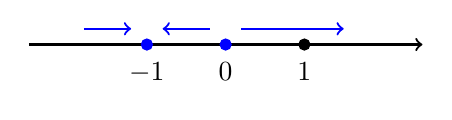
\begin{tikzpicture}
        % Eje
        \draw[->, thick] (-2.5,0) -- (2.5,0);
        
        % Puntos de equilibrio
        \filldraw[blue] (-1,0) circle (2pt) node[below=3pt, text=black] {$-1$};
        \filldraw[blue] (0,0) circle (2pt) node[below=3pt, text=black] {$0$};
        \filldraw[black] (1,0) circle (2pt) node[below=3pt] {$1$};
        
        % Flechas de dinámica
        \draw[->, thick, blue] (-1.8,0.2) -- (-1.2,0.2);
        \draw[<-, thick, blue] (-0.8,0.2) -- (-0.2,0.2);
        \draw[->, thick, blue] (0.2,0.2) -- (1.5,0.2);
    \end{tikzpicture}
    \end{center}
}

% Ejercicio 7
\ejercicio{enunciado}{}{
    Dados $\lambda > 0$, $\mu > 0$, $b > 0$, y $c > 0$, considera el modelo de especies competitivas:
    \[
        \begin{cases}
            u' = \lambda u - u^2 - buv, \\
            v' = \mu v - v^2 - cuv,
        \end{cases}
        \quad (u(0), v(0)) = (u_0, v_0),
    \]
    donde $u_0 \ge 0$ y $v_0 \ge 0$.
    \begin{enumerate}[label=(\alph*)]
        \item Demuestra que el sistema tiene una única solución maximal a la derecha, $(I, u, v)$.
        \item Determina la solución maximal cuando $u_0 = 0$ o $v_0 = 0$.
        \item Demuestra que $u(t) > 0$ y $v(t) > 0$ para todo $t \in I$ si $u_0 > 0$ y $v_0 > 0$.
        \item Demuestra que $I = [0, \infty)$ si $u_0 > 0$ y $v_0 > 0$.
    \end{enumerate}
}{}

% Ejercicio 8
\ejercicio{enunciado}{}{
    Repite el ejercicio anterior para el modelo depredador-presa, que viene dado por:
    \[
        \begin{cases}
            u' = \lambda u - u^2 - buv, \\
            v' = \mu v - v^2 + cuv,
        \end{cases}
        \quad (u(0), v(0)) = (u_0, v_0),
    \]
    donde $\lambda > 0$, $\mu > 0$, $b > 0$, $c > 0$, $u_0 \ge 0$, y $v_0 \ge 0$.
}{}

% Ejercicio 9
\ejercicio{enunciado}{}{
    Dados $\lambda > 0$ y $b > 0$, considera el modelo simbiótico:
    \[
        \begin{cases}
            u' = \lambda u - u^2 + buv, \\
            v' = \lambda v - v^2 + buv,
        \end{cases}
        \quad (u(0), v(0)) = (1, 1).
    \]
    Demuestra que admite una única solución maximal a la derecha. Determina esta solución y su tiempo maximal de existencia en términos del parámetro $b > 0$, el cual mide la sinergia entre los individuos de las especies $u$ y $v$.
}{}

% Ejercicio 10
\ejercicio{enunciado}{}{
    Dado el sistema plano:
    \[
        \begin{cases}
            u' = u + v - u(u^2 + v^2), \\
            v' = -u + v - v(u^2 + v^2),
        \end{cases}
    \]
    obtén un sistema equivalente utilizando coordenadas polares, $u = \rho \cos \theta, \quad v = \rho \sin \theta$. Resuelve el sistema resultante y representa las soluciones del sistema original en el plano $(u,v)$.
}{}

% Ejercicio 11
\ejercicio{enunciado}{}{
    Dados $p > 0$ y $q > 0$ con $pq < 1$, considera el problema:
    \[
        \begin{cases}
            u' = |v|^p, \\
            v' = |u|^q,
        \end{cases}
        \quad (u(0), v(0)) = (1, 1).
    \]
    Demuestra la existencia de una única solución maximal a la derecha, $(I, u, v)$, y analiza su carácter global.
}{}

% Ejercicio 12
\ejercicio{enunciado}{}{
    Dados $h, j, k, \ell \in \N \setminus \{0\}$, demuestra que, para todo $t_0 \in \R$ y $(u_0, v_0) \in \R^2$, el problema:
    \[
        \begin{cases}
            u' = -u^{2h+1} v^{2\ell}, \\
            v' = -u^{2j} v^{2k+1},
        \end{cases}
        \quad (u(t_0), v(t_0)) = (u_0, v_0),
    \]
    tiene una única solución, la cual está globalmente definida en $[t_0, \infty)$.
}{}

% Ejercicio 13
\ejercicio{enunciado}{}{
    Se dice que una función $f \in \mathcal{C}^1(\R \times \R^N; \R^N)$ es del \textit{tipo de Kolmogorov} si, denotando $u = (u_1, \dots, u_N)^T$ y $f = (f_1, \dots, f_N)^T$, existen funciones $g_i \in \mathcal{C}(\R \times \R^N; \R)$, con $1 \le i \le N$, tales que
    \[
        f_i(t,u) = g_i(t,u)u_i \quad \text{para todo } i \in \{1, \dots, N\}, t \in \R, u \in \R^N.
    \]
    Asumiendo que $f$ es del tipo de Kolmogorov, considera, para todo $u_0 \in \R^N$, el problema de valor inicial:
    \[
        \begin{cases}
            u' = f(t,u), \\
            u(0) = u_0.
        \end{cases}
    \]
    \begin{enumerate}[label=(\alph*)]
        \item Demuestra la existencia de una única solución maximal y discute todos sus comportamientos admisibles.
        \item Sea $(I, u(\cdot; u_0))$ la solución maximal. Demuestra que $\text{signo } u_i(t; u_0) = \text{signo } u_{0i}$ para todo $t \in I$ e $i \in \{1, \dots, N\}$, donde $u_0 = (u_{01}, \dots, u_{0N})^T$.
        \item Supón que, adicionalmente, $g_i(t, u) = \lambda_i - \sum_{j=1}^N a_{ij} u_j$, para $1 \le i \le N$, donde $\lambda_i \in \R$ y $a_{ij} \ge 0$ son constantes para cada $i,j \in \{1, \dots, N\}$. Demuestra que, en tal caso, $u(t;u_0)$ está globalmente definida en $[0, \infty)$ siempre que $u_{0i} \ge 0$ para todo $i$. Asumiendo, además, que $\lambda_i < 0$ para todo $i$, demuestra que $\lim_{t \to \infty} u_i(t) = 0$.
        \item Da ejemplos, con $N=2$ y $a_{12} = a_{21} < 0$, para los cuales la solución explote en tiempo finito.
    \end{enumerate}
}{}

% Ejercicio 14
\ejercicio{enunciado}{}{
    Dado un entero $N \ge 1$ y una matriz cuadrada no nula $A = (a_{ij})_{1\le i,j \le N} \in \mathcal{M}_N(\mathcal{C}(\R; \R))$, considera la función $f(t,u) = (f_1(t,u), \dots, f_N(t,u))^T$, con $u = (u_1, \dots, u_N)^T$, cuyas componentes se definen como
    \[
        f_i(t,u) = \sum_{j=1}^N a_{ij}(t)|u_j|^{p_{ij}}, \quad (t,u) \in \R \times \R^N, \;\; 1 \le i \le N,
    \]
    donde, para cada $i,j \in \{1, \dots, N\}$, $p_{ij} \ge 1$. Demuestra la existencia y unicidad de una solución maximal para el problema
    \[
        \begin{cases}
            u' = f(t,u), \\
            u(0) = u_0 \in \R^N.
        \end{cases}
    \]
    Discute todos sus comportamientos admisibles, y da ejemplos para todos ellos en el caso particular $N=2$ eligiendo apropiadamente $a_{ij}(t)$ y $p_{ij}$.
}{}

% Ejercicio 15
\ejercicio{enunciado}{}{
    Demuestra que, para todo $\varepsilon \ge 0$, el problema
    \[
        \begin{cases}
            u'(t) = t [\sin u(t) + \varepsilon \cos u(t)], \\
            u(0) = 1,
        \end{cases}
    \]
    tiene una única solución globalmente definida en $[0, \infty)$, denotada por $u_\varepsilon$, y estima $|u_\varepsilon(t) - u_0(t)|$ para todo $t > 0$ y $\varepsilon > 0$.
}{}

% Ejercicio 16
\ejercicio{enunciado}{}{
    Demuestra que, para todo $\varepsilon \ge 0$, el problema
    \[
        \begin{cases}
            u'(t) = t \sin u(t), \\
            u(0) = \varepsilon,
        \end{cases}
    \]
    tiene una única solución globalmente definida en $[0, \infty)$, denotada por $u_\varepsilon$, y estima $|u_\varepsilon(t) - u_0(t)|$ para todo $t > 0$ y $\varepsilon > 0$.
}{}